
    \begin{abstract_online}{Molecular Dynamics Simulation of Anti-HIV Protein SAMHD1 }{%
        \underline{G. Thapa}, S. Bhattacharya}{%
        }{%
        Department of Chemical Engineering, IIT Kanpur, India}
    The human sterile alpha motif and HD domain-containing protein 1 (SAMHD1)  is a retroviral restriction factor in myeloid cells and non-cycling CD4+ T  cells, a feature imputed to its phosphohydrolase activity – the enzyme  depletes the cellular dNTP levels inhibiting reverse transcription. The  functionally active form of SAMHD1 is an allosterically triggered tetramer  which utilizes $GTP$-$MG^{+2}$-$dNTP$ cross bridges to link and stabilize adjacent monomers. \par  Our target is to unravel the restriction mechanism and, in particular,  elucidate the allosteric and regulatory mechanisms of the protein. Strangely, phosphorylation studies at T592 residue has shown loss in HIV-1  restriction ability but no correponding loss in the dNTPase activity. This  does not correlate well with the proposed mechanism of HIV-1 restriction.  So it is anticpated that other mechanisms of antiviral restriction by  SAMHD1 might occur in the cell. A study has found that mutated dimeric  form of  pig SAMHD1 is capable of dNTPase activity. In this study we  carried out molecular dynamics simulations of dimeric form of human SAMHD1  to uncover the mechanism of antiviral restriction by SAMHD1.  \begin{center}  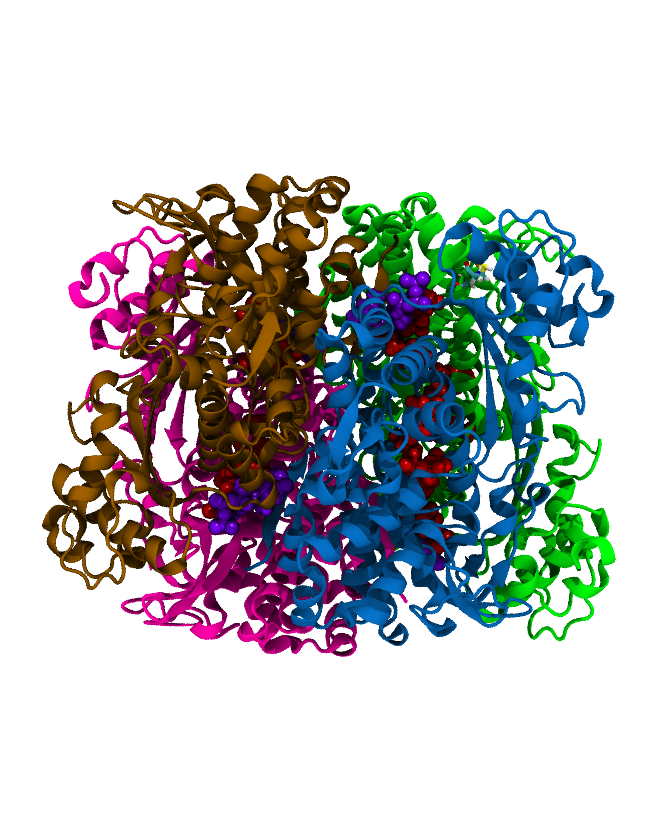
\includegraphics[scale=0.3]{abstracts/txt/figures/thapa1.png}  \caption{\textbf{Figure 1:} SAMHD1 tetramer}  \end{center} \begin{center}  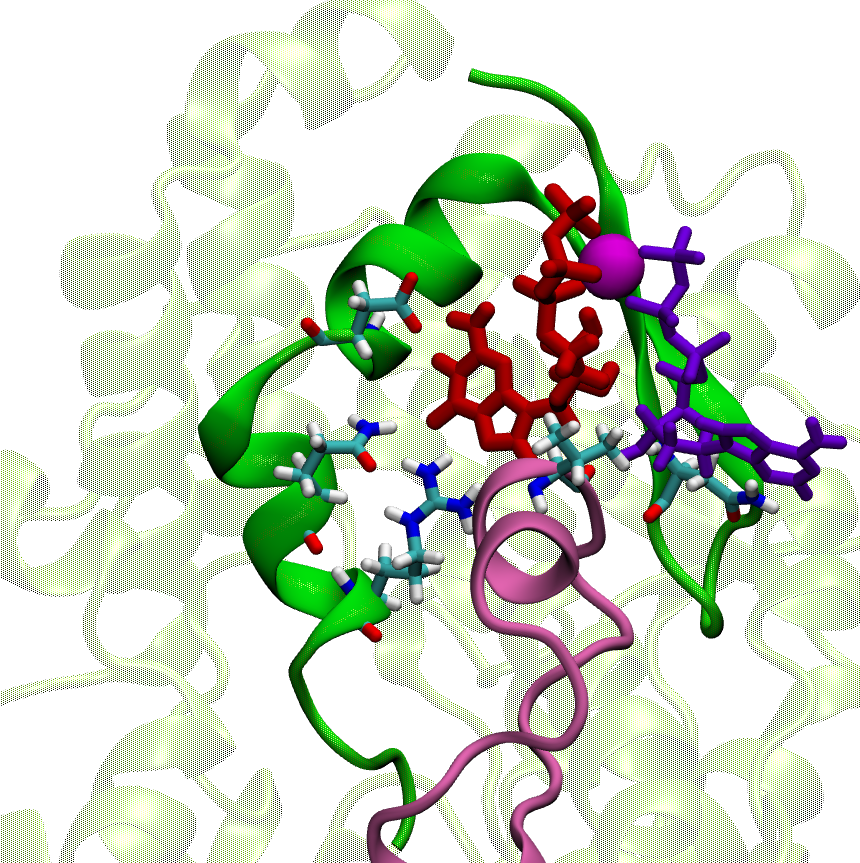
\includegraphics[scale=0.3]{abstracts/txt/figures/thapa2.png}  \caption{\textbf{Figure 2:} $GTP$-$MG^{+2}$-$dNTP$ cross bridge}  \end{center} 
    
        \textbf{References} \newline{}[1] Christopher H. Mauney & Thomas Hollis, Autoimmunity, 51:3 (2018),  96-110\newline{}[2] Xiao-Hong Qin, Febs J., 286:19 (2019), 3844-3857
    \end{abstract_online}
    